% \chapter{Case Study and Discussion}
\chapter{案例分析与讨论}
\label{chp:casestudy}
% In this section, we present some samples in our dataset, not only to firm our findings but also to provide more valuable insights.
在本章中,我们会呈现数据集中的一些样本,不仅仅是为了确认我们在上一章中提及的各种发现,同时也是为了提供一些更有价值的见解,让读者对我们的数据集、对仿冒应用有更加深刻的认知。

% \noindent{\bf Case study 1.} \emph{Fake certificate with multiple malicious imitators and imposters}
\section{案例 1. 与大量仿冒应用相关联的仿冒应用安全证书}
\label{sec:case1}

% We manually review the samples signed by the certificate with SHA1 ``\emph{61ed377e85d386a8dfee6b864bd85b0bfaa5af81}", the certificate with the most number of fake samples among our fake certificate set (i.e., 1,374 fake samples).
在\secref{sec:fakeCharacteristics}中,我们提到有部分仿冒应用安全证书关联着多个仿冒样本。
其中,一个SHA1码为``\emph{61ed377e85d386a8dfee6b864bd85b0bfaa5af81}''的安全证书是所有证书中关联仿冒样本最多的,足足有1,374个样本持有这个仿冒证书。
% On top of that, this certificate is also one of the certificates survive the longest time (nearly 3 years) and is still active.
不仅如此,这个安全证书还是其中一个在应用市场中存活时间最长的仿冒应用安全证书。
它的出现横穿了我们的整个研究时间过程(接近三年),而且在我们的数据收集流程结束前依然呈现活跃状态。

% Originally, we presume this certificate to belong to a benign app which passes the verification of analysts in Pwnzen, since the number of samples it links to even exceeds the number of official samples of some apps.
最初,我们假定这个证书属于某个通过犇众分析团队验证的良性应用,因为它关联的样本数量实在是太大了,这个数量甚至超过了我们某些目标App的样本总量。
% The truth is, however, after manually review, we found all the 1,374 samples linked with this certificate are typical fake samples, in form of either imitators or imposters, covering 79\% (37 out of 47) of our target apps.
然而在人工审核之后,我们却发现了意料之外的结果。
这个证书关联的所有1,374个样本都是典型的仿冒样本,其中既有只与原版应用稍微近似的\texttt{模仿应用},也有外观上完全模仿原版应用的\texttt{高仿应用},覆盖了我们能找到的47个目标App中的37个(79\%)。
% Some of its samples can even be organized in version order, which means the developer does track official apps to update its fake versions as maintenance.
而这些证书关联的一些样本,甚至有自己的版本顺序,这表明有的开发者真的会追踪官方App的各个版本来更新、甚至维护自己的仿冒版本。

\begin{table}[htbp]
	\renewcommand{\arraystretch}{1}
	\small
	\centering
	\caption{由``61ed377e85d386a8dfee6b864bd85b0bfaa5af81"签署的部分样本}
	\vspace{1mm}
	\rowcolors{2}{gray!15}{white}
	\begin{tabular}{l l c c c c c c}
		\toprule
		{\bf Name} & {\bf Package Name} & {\bf Size} \\
		\midrule
		QQ Talk  & net.in1.smart.qq & 465.8 KB \\
		QQ  & com.h & 8.2 MB \\
		爱微信  & com.lovewechat & 368.4 KB \\
		微信  & com.tencen1.mm & 22.1 MB \\
		UC Mini  & com.uc.browser.en & 2.1 MB \\
		UC 浏览器  & com.UCMobile.microsoft & 21.3 MB \\
		Clean Master  & com.blueflash.kingscleanmaster & 972.0 KB \\
		WiFi万能钥匙  & com.snda.wifilocating & 5.9 MB \\
		\bottomrule
	\end{tabular}
	\label{table:certificate_case_study}
\end{table}

% We display some of the samples singed by this certificate in Table~\ref{table:certificate_case_study}, they are all reported to be malicious (i.e., Ad-ware, spyware or Trojan) on \textsc{Virustotal}~\cite{virustotal}, a famous online antivirus engine.
我们在\autoref{table:certificate_case_study}中展现了由这个安全证书签署的部分样本。
我们将这些样本上传到知名在线反病毒引擎\textsc{Virustotal}~\cite{virustotal}上,结果显示,与该证书关联的所有样本都是恶意样本(广告软件、间谍软件或木马软件等)。
% So far the samples related to our target apps have already been showing up in 20 markets including the leading ones like \texttt{\small Myapp} and \texttt{\small Qihoo 360 Market}.
到目前为止,由这个证书签署的仿冒样本已经在我们的20个应用来源(即应用市场)中出现,包括\texttt{应用宝}和\texttt{360应用市场}等主流应用市场。
% What's more, \texttt{\small Baidu App Store} keeps receiving apps with this certificate from 2015 to recently -- its latest ``product'' was put on shelf on September 15$^{th}$, 2018.
除此之外,\texttt{百度手机助手}从2015年起就开始接受由这个安全证书签署的应用,直到我们的数据收集阶段结束前——数据显示,这个安全证书在2018年9月15日还在\texttt{百度手机助手}上架了一款应用。

% To this end, we can draw the following conclusions:
在这里,我们可以得到以下两个结论:
\begin{itemize}
	% (1) Even the leading app markets (and the top developers) are unqualified in detecting malicious apps.
	\item 就算是领先的应用市场(和顶尖的开发者)在检测恶意应用方面也不能做到尽善尽美,而现有的检测方法也有所不足,未能及时地找出可疑的开发者;
	% (2) Existing app markets lack information exchange on defending attacks from underground industry.
	\item 从这个证书在多个市场都存在的现象,我们可以推导,现有的应用市场缺乏有效的信息交换机制。如果各个应用市场能建立一个互通信息的平台,分享可疑开发者/恶意开发者信息,那么将可以杜绝一部分恶意开发者在各个应用市场上到处流窜的现象。
\end{itemize}

% \noindent{\bf Case study 2.} \emph{Fake samples in different gaming apps}
\section{案例 2. 游戏类别下的仿冒应用}

% Gaming apps in our target app list (i.e. \texttt{\small ArenaofValor} and \texttt{\small HappyElements}) attract a number of fake samples.
正如\autoref{table:data-statistics}中数据所示,\texttt{游戏}类应用(\texttt{王者荣耀}和\texttt{开心消消乐})吸引了大批的仿冒应用样本。
% To figure out what do these samples look like, we randomly downloaded some of the fake samples of the 2 gaming apps (7 samples for each) and installed them on our testing device.
出于性能考虑,我们的数据中只提取了APK包的基本信息,并没有对收集到的每个APK文件进行详细的分析。
因此,为了弄清楚这些仿冒应用究竟是怎么样的,我们随机从这两款游戏App的仿冒样本中选择了一些样本(每款应用选择7个仿冒样本),然后将这些样本安装到了我们的实验设备上。

% Fig.~\ref{fig:screenshot_all} shows how these samples look like on a real Android phone, official apps are marked with green frames.
\autoref{fig:screenshot_all}展示了这些样本在真实的Android设备上安装之后的实际外观。
官方渠道下载的正版App在图片中由绿色边框标记出。
% Apparently, fake samples have either a similar name or a similar icon to official ones.
明显地,我们能看到,与官方应用相比,仿冒应用要么就有一个和官方应用名十分相似的应用名,要么就在图标上和官方相近甚至相同。

\begin{figure}[htbp]
	\centering
    \subfloat[两种游戏App与其仿冒\label{fig:screenshot_all}]{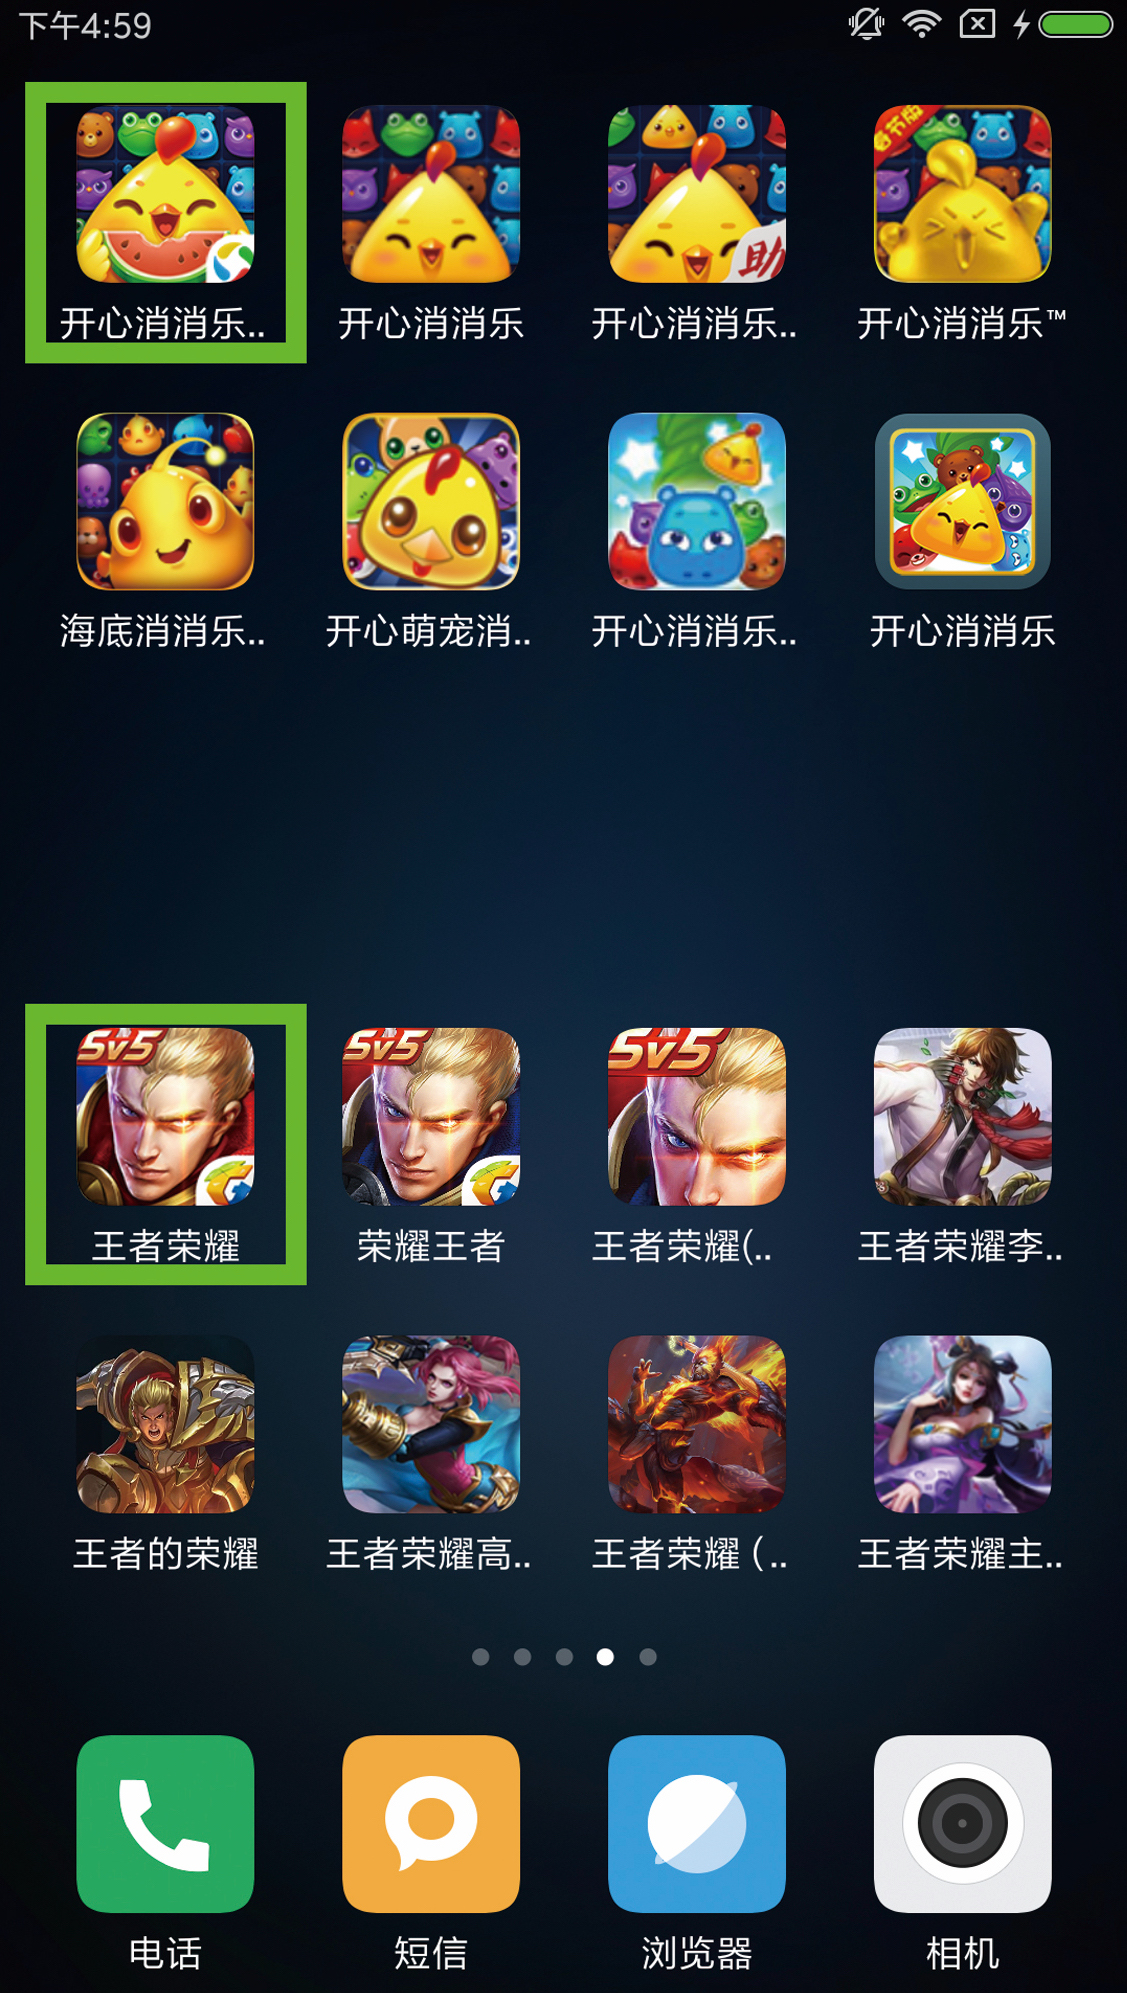
\includegraphics[width=0.3\textwidth]{./Figures/edwin-screenshot1.jpg}}\hfill
    \subfloat[正版\textit{\small 开心消消乐}\label{fig:screenshot_official}]{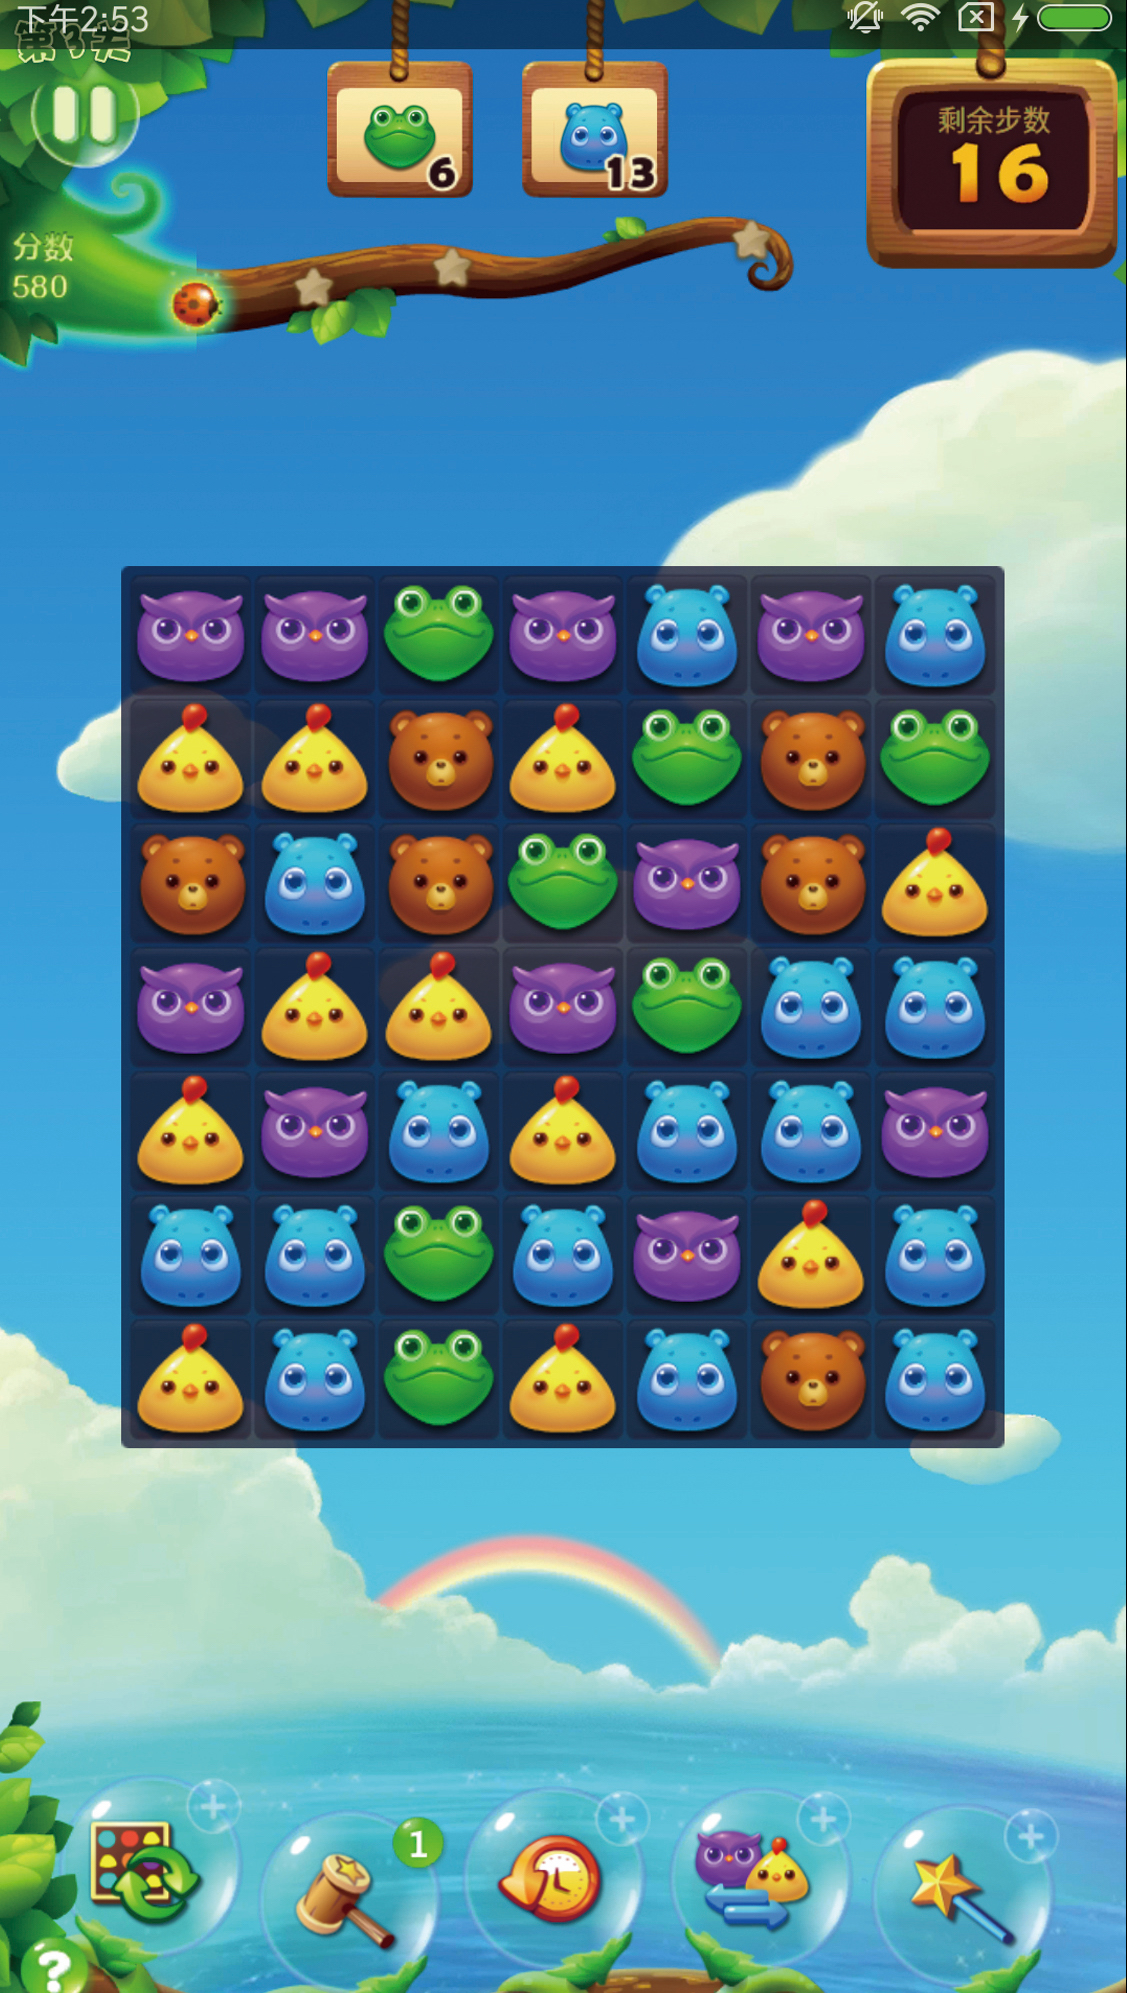
\includegraphics[width=0.3\textwidth]{./Figures/edwin-screenshot2.jpg}}\hfill
    \subfloat[仿冒版\textit{\small 开心消消乐}\label{fig:screenshot_fake}]{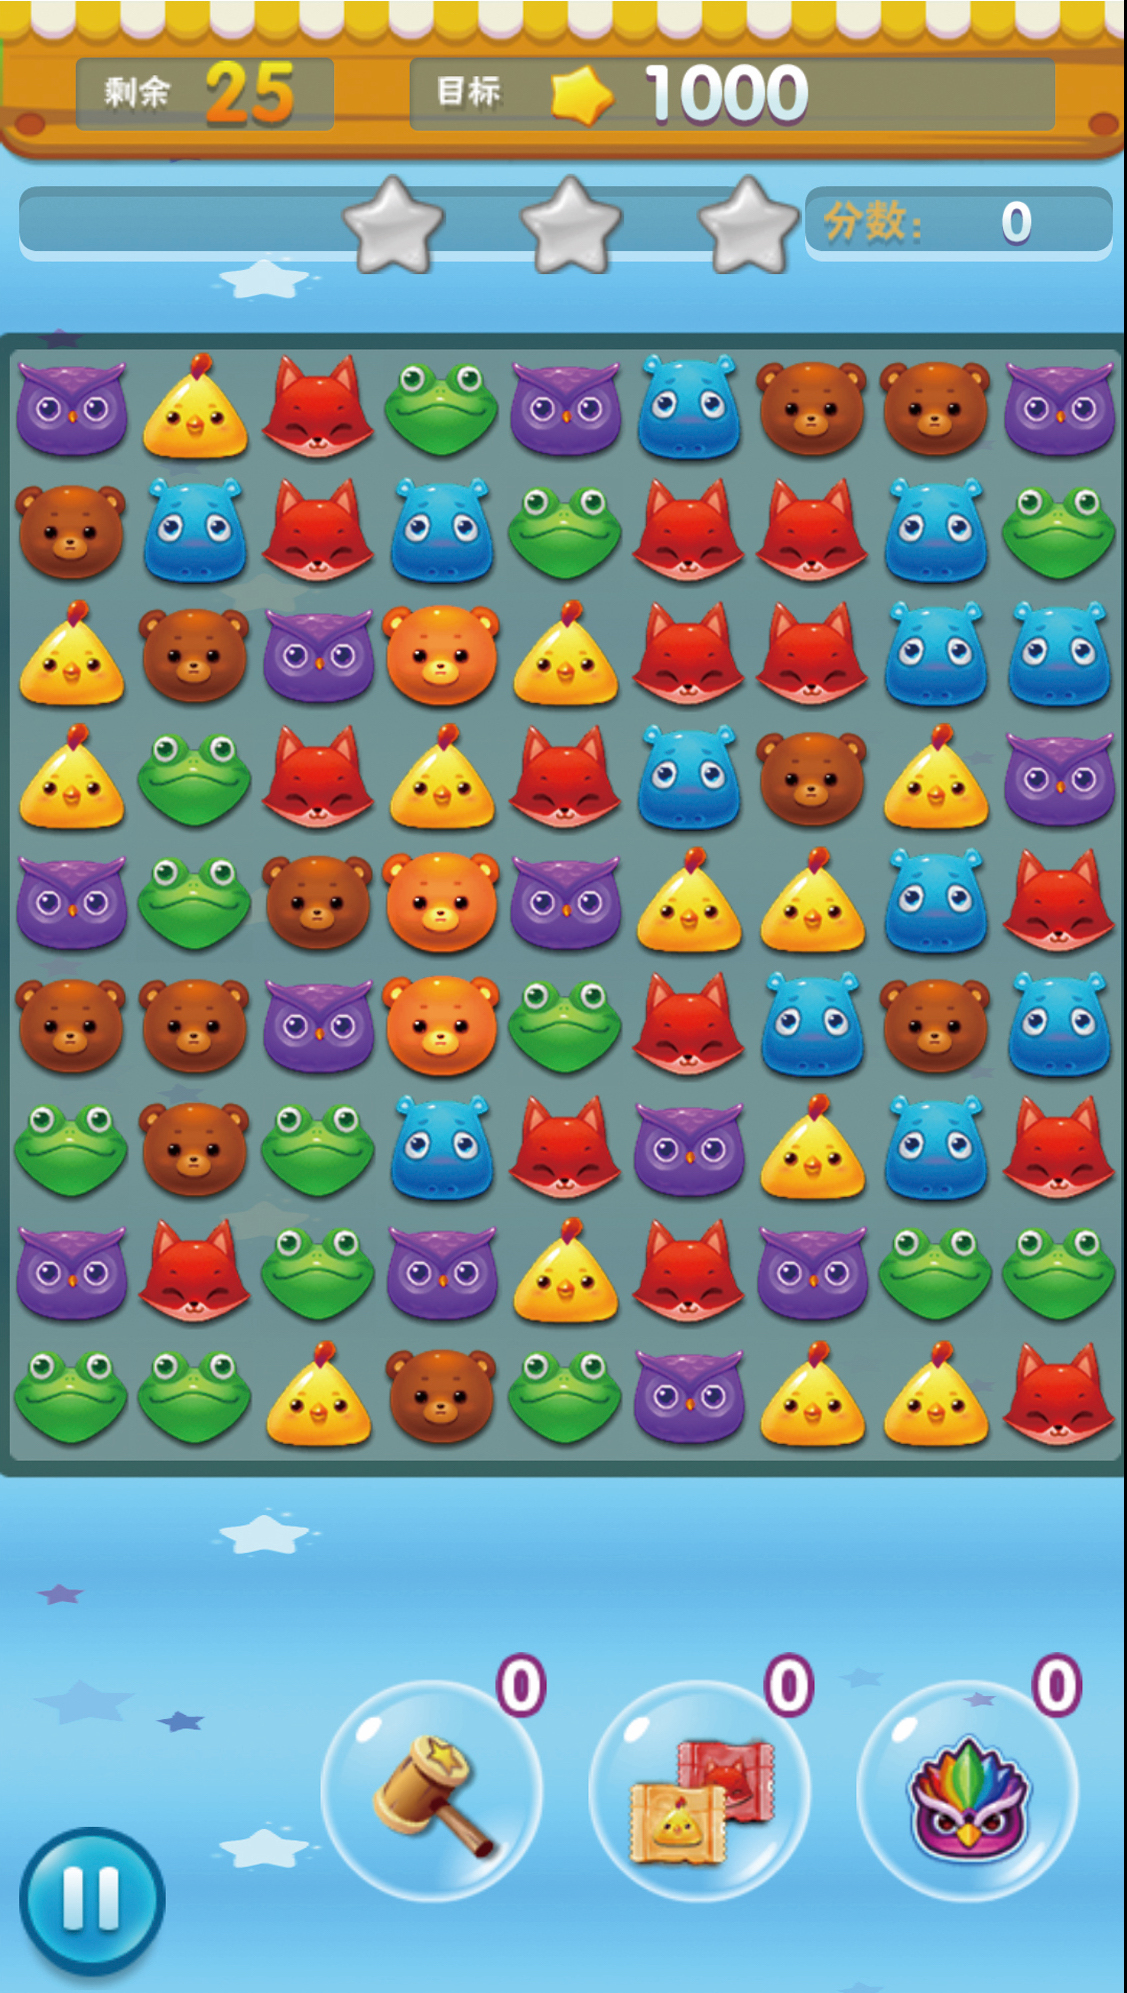
\includegraphics[width=0.3\textwidth]{./Figures/edwin-screenshot3.jpg}}\hfill
    \caption{游戏类App及其仿冒样本}
\end{figure}

% We even ran these apps on our device.
我们甚至在测试设备上实际运行了上述安装的14个仿冒样本,然后拿他们和原版的应用对比。
我们使用的测试设备是高配版的小米5手机,搭载的CPU为最高主频2.15GHz的骁龙820处理器,3GB内存,64GB机身存储,安装的Android系统版本为Android 6.0(Android Marshmallow,API 23)。

% Screenshots were captured when we ran one of the fake samples (see Fig.~\ref{fig:screenshot_fake}) and the official sample (Fig.~\ref{fig:screenshot_official}).
\autoref{fig:screenshot_official}和\autoref{fig:screenshot_fake}分别是在我们在测试设备上运行官方版本的\texttt{开心消消乐}和其中一个仿冒版的\texttt{开心消消乐}时的系统截屏。
不难看出,两款应用的外观是十分相像的。
我们在测试时发现,两款游戏内部的玩法、实际操作逻辑也一模一样。
如果不是事先知道了哪一款应用是来自官方渠道下载的正版,连我们都没有办法判别两个应用的真伪,更不必说是从应用市场搜索结果中找到这些结果的普通用户了。

% As a result, we found that 4 fake samples of \texttt{\small HappyElements} are actually games that are similar to the official one (one is a repackaged app with high confidence), 2 are raiders on the game and the last one crashed when it was launched.
而这并不是唯一的案例。作为结果,我们发现7款\texttt{开心消消乐}的仿冒样本中,有4款是与官方样本十分相似的游戏(其中一个十分可能是经过重打包技术处理的应用),2款声称自己是``系统攻略'',还有1款在运行时闪退,无法在我们的设备上实际运行。
% 3 out of the 4 fake games pop up alert windows in the game to require users for In-App purchase, which is very possible to cause unwilling cost.
在4款仿冒游戏中,3款都在游戏中不时自动弹出游戏内购窗口,要求玩家购买道具,十分可能导致玩家不想要的花费。
% All 7 samples are reported to be malicious on \textsc{Virustotal}~\cite{virustotal}.
而所有7个仿冒样本都在\textsc{Virustotal}~\cite{virustotal}中被报告为恶意应用。

% Fake samples on \texttt{\small ArenaofValor}, in contrast, barely have functionalities like the official one.
相比之下,\texttt{王者荣耀}的仿冒样本内容就与官方应用大相径庭了。
% 3 of those samples are wallpaper setters and the rest 4 are simply puzzle games.
在7款被安装到测试设备的仿冒样本中,有3款是壁纸浏览器,里面包含了几张游戏内人物的插画,可以在应用内将这些插画设置成系统的桌面壁纸;
而余下四个是简单的拼图游戏,里面同样包含了王者荣耀游戏人物的插画,应用内容就是简单地把被打乱的插画拼图恢复原状。
% Virustotal reports 6 out of the 7 samples as malware, the last one is claimed as potentially unwanted program (PUP).
Virustotal的结果显示,7款仿冒样本中,有6款是恶意软件,涵盖了木马病毒、广告软件等类型,而余下的一款则被报告为潜在有害程序(Potentially Unwanted Program,简称PUP)。
PUP通常在用户不知情或者不愿意的情况下,通过静默安装或者捆绑安装的形式被安装在系统中。
尽管这种软件不一定包含恶意代码,但其动机十分可疑。

% We determine it is the difficulty to imitate the official app's functionality that brings about this phenomenon.
我们认为,这种现象是由模仿正版应用功能的难易程度带来的。
% The core implementation of multiplayer online battle arena (MOBA) games like \texttt{\small ArenaofValor} is much more complicated than that in \texttt{\small HappyElements}.
只从技术角度看,像\texttt{王者荣耀}这样的多人在线战斗竞技场(Multiplayer Online Battle Arena,简称MOBA)游戏核心难度明显要比\texttt{开心消消乐}这样的益智类游戏要高得多。
一款MOBA游戏除了要解决支持运行运行的物理引擎之外,还要实现聊天系统、在线匹配、负载均衡等业务,更加不必说背后的人物设计技能平衡等更深入的话题了;而一款益智类三三消游戏的核心逻辑就只在于元素三连的判定和随机新出现的元素,再加上道具系统就差不多可以包装成一个完整的游戏推出。

% What it costs to develop a complex game like \texttt{\small ArenaofValor} is exorbitant for a fake developer.
因此,就算不考虑后续的维护问题,要开发一款像\texttt{王者荣耀}这样的复杂游戏,对仿冒应用开发者来说明显是成本过高的。
但由于这款游戏本身具有超高的热度,可能带来巨大的收益,所以仿冒应用开发者会为了蹭上热度而开发外观相似、内容完全不符的仿冒样本。
相比之下,\texttt{开心消消乐}由于开发难度相对较小,所以仿冒应用开发者会愿意开发一个内容相似的应用,再通过内购陷阱等手段收取效益。
这两款App透露出了仿冒应用开发者在仿冒方面两个截然不同的思路。

% Therefore, we can infer another reason why apps in \texttt{\small productivity} category gain a low fake sample rate:
我们在\secref{sec:quantitativeStudy}中观察到的\texttt{商务办公}类别有较低仿冒率也可能是类似原因导致的结果。
% Unlike games, on one hand, productivity tools are less likely to have peripheral products (like wallpaper setter mentioned above);
一方面,\texttt{商务办公}类的工具核心逻辑比较复杂,对仿冒开发者来说并不是一个有利可图的最佳选项;
% On the other hand, the inevitably laborious developing procedure also prevents the tools themselves from being shammed.
另外,这类应用也不像\texttt{游戏}一样会衍生出周边产品(比如\texttt{王者荣耀}的游戏人物就会有不少插画),仿冒应用开发者也没办法从这方面入手蹭热度。
结合两个原因,\texttt{商务办公}类的应用自然就不会引起仿冒应用开发者的太多兴趣了。

% \noindent {\bf Case study 3.} \emph{Suspicious samples with official certificate}
\section{案例 3. 持有官方安全证书的可疑样本}

% Case study 1 gives us a perfect example on counterintuitive data in our data set.
\secref{sec:case1}的案例1提供了我们数据集中一个明显反直觉的示例。
% In order to find out whether or not resemble cases exist in our official samples, we manually reviewed them and noticed a weird entry when sorting out the sample log, a sample claims itself to be ``cracked" in its app name.
因此,我们不禁会好奇数据集中是否会有其他违反直觉的数据存在。
为了解开这个疑问,我们决定先从搜集到的正版样本入手。
我们手动浏览了所有69,614个持有官方证书的样本,其中有一个样本的应用名十分可疑——该样本声称自己是一个``破解版''的应用。
% Furthermore, we checked (1) if strange word (e.g., ``cracked") appears in our official samples' names, (2) whether or not an official app is signed by an official certificate from another developer, and (3) if one official sample has a suspicious package name.
于是,我们再次针对所有正版样本进行了以下几项筛选:
\begin{enumerate}
	\item 使用``破解''、``免费''等关键字搜索所有带正版证书的样本,筛选出带有可疑应用名的样本;
	\item 筛选所持安全证书与原开发者不一致的样本;
	\item 筛选出包名和同款App的多数样本不一致的样本。
\end{enumerate}

% Eventually we acquired 17 suspicious official samples, listed in table~\ref{table:suspicious_samples} are samples in each of these three kinds.
最终,我们获得了17个由正版开发者安全证书签署的可疑样本,其中三个样本的信息如\autoref{table:suspicious_samples}中所示,分别代表上述三项筛选得到的结果。
第一个名为\texttt{爱奇艺}的样本虽然由一个官方安全证书签名,但该安全证书和其他爱奇艺样本的却不一致。对比之后,我们发现该证书来自360手机助手,但360和爱奇艺并没有合作关系,因此这是个可疑的样本;
而第二个样本(\texttt{360手机助手})的可疑之处在于样本包名。多数\texttt{360手机助手}的包名为\emph{com.qihoo.appstore},也有少部分官方包名为\emph{com.qihoo.secstore},前者为\texttt{360手机助手}在国内第三方应用市场发行的应用包名,后者为Google Play官方应用市场上上架的包名。然而,其中一个使用了其官方安全证书签署的样本的包名却是\emph{com.kuyou.sdbgj.baidu},十分奇怪;
第三个样本则是在应用名中包含了``破解''字样。然而,正常的正版应用根本不会有这样的命名方式,所以我们也认为这是一个可疑样本。

% \textsc{Virustotal} reports that only 2 of the 17 samples are benign, 2 are PUP and the other 13 samples are all malicious.
\textsc{Virustotal} 的检查结果显示,17个可疑样本中,只有2个是良性应用,2个是PUP,余下13个样本都被判定具有恶意行为。

\begin{table*}[htbp]
	\renewcommand{\arraystretch}{1}
	\small
	\centering
  \setlength{\belowcaptionskip}{-10pt}
	\caption{持有官方安全证书的可疑样本}
	\begin{tabular}{l l c c c c c c}
		\toprule
		{\bf 样本应用名} & {\bf 样本SHA1码} & {\bf 可疑之处} \\
		\midrule
		% 爱奇艺 & b86c55a509e8293b24138b166e9ff410f39e84b5 & 可疑证书(360手机助手) \\
		爱奇艺 & b86c55a509e8293b24138b166e9ff410f39e84b5 & 可疑证书\\
		% 360手机助手 & 2bb43c53b86d204d0040a8af6cb2a09cf9e93bb7 & 可疑包名(com.kuyou.sdbgj.baidu) \\
		\rowcolor{gray!15} 360手机助手 & 2bb43c53b86d204d0040a8af6cb2a09cf9e93bb7 & 可疑包名\\
		% Youku XL 破解版 & b55b7ef189d649aeb03443c5d1ab57c9031d624e & 可疑应用名(``破解版") \\
		Youku XL 破解版 & b55b7ef189d649aeb03443c5d1ab57c9031d624e & 可疑应用名 \\
		\bottomrule
	\end{tabular}
	\label{table:suspicious_samples}
\end{table*}

% Despite the possibility that these certificates were somehow leaked to the underground industry, it is more likely that some attackers penetrated the protection scheme.
鉴于这17个样本都是持有官方安全证书签名的,我们起初不禁怀疑是否有应用厂家不慎泄露了自己的安全密钥库,从而导致了这些样本的出现。
然而,如果真的是因为厂家泄露密钥库,一来很有可能会导致恶意开发者使用官方安全证书大量生产恶意应用,二来对应厂家也会出于安全考虑马上更换新的包名和安全证书。
我们的数据并不支持以上猜想带来的两点结果,所以我们不认为这是由于安全证书泄露导致了这些可疑样本的产生。

除去这个可能性,我们认为更有可能的原因是某些仿冒应用开发者掌握了穿透/绕过Android系统签名机制的技术,从而产生了这些样本。

% As far back as December 2017, Google had confirmed and revealed a backdoor on V1 signature scheme (CVE-2017-13156)~\cite{android_security_bulletin}, by which hackers can inject any content into an apk at will without modifying its certificate information.
时间回溯到2017年12月,Google确认并公布了V1版本应用签名机制的一个后门(CVE-2017-13156)~\cite{android_security_bulletin}。
通过这个后门,黑客可以在不修改APK包安全证书信息的情况下,向APK包里注入任意内容。
% An alternative solution, V2 signature scheme, has been launched at least one year before that.
而早在这个漏洞被公布的至少一年之前,Google就已经发布了作为V1版签名机制的替代解决方案,也就是V2版应用签名机制。
% In order to confirm if these apps are using the risky V1 scheme, we used a tool, \textsc{apksigner}, provided by Google to verify which signature schemes these samples are using.
这看起来十分有可能是导致这些可以样本产生的原因,某些恶意开发者利用了V1版本签名机制的漏洞,修改了APK包的基本信息。
为了确认这些样本是否采用了具有风险的V1版应用签名机制,我们使用了\textsc{apksigner}来检测这些样本使用的签名机制版本。
\textsc{apksigner}是Google官方提供的一个命令行工具,它被集成在Android SDK中,既是APK包编译打包过程中为APK包进行数字签名的工具,也可以用来验证APK包使用的签名机制版本,又或者是验证APK的签名是否有效。

% It ends up that all 17 samples are using V1 signature scheme.
\textsc{apksigner}的结果显示,所有17个样本都只使用了V1版本的应用签名机制。
% With actually knowing that V1 is no longer safe, developers still refuse to embrace the safer scheme, which is really disappointing.
在了解到V1版本签名机制已经不再安全的情况下,仍有部分开发者由于各种原因没有接受更新也更安全的签名方案,这个结果有点令人失望。

\section{本章小结}
本章从数据集中选出了一些较有代表性又或者反直觉的数据样本,为读者提供了3个不同的案例分析,在为我们在上一章的发现提供有力支持之外,也揭示了更多仿冒应用开发者的行为特征。
回看三个案例,我们不难发现,仿冒应用开发者的确会抓住一切可能的机会,利用包括签名机制漏洞、市场审查机制缺陷在内的各种办法制作出仿冒甚至是恶意应用。
同时,本章的三个案例也说明了无论是开发人员还是应用市场,都应该为保护Android的软件安全上投入更大精力,从而更好地防范来自移动黑产的各种攻击。
